\section{The Fundamental Theorem of Calculus}\label{sec:FTC}
Let's recast the first example from the previous section. Suppose that
the speed of the object is $3t$ at time $t$. How far does the object
travel between time $t=a$ and time $t=b$? We are no longer assuming
that we know where the object is at time $t=0$ or at any other
time. It is certainly true that it is {\it somewhere,} so let's
suppose that at $t=0$ the position is $k$. Then just as in the
example, we know that the position of the object at any time is 
$\ds 3t^2/2+k$. This means that at time $t=a$ the position is 
$\ds 3a^2/2+k$ and at time $t=b$ the position is $\ds 3b^2/2+k$. Therefore the
change in position is $\ds 3b^2/2+k-(3a^2/2+k)=3b^2/2-3a^2/2$. Notice that
the $k$ drops out; this means that it doesn't matter that we don't
know $k$, it doesn't even matter if we use the wrong $k$, we get the
correct answer. 

What about the second approach to this problem, in the new form? We
now want to approximate the change in position between time $a$ and
time $b$. We take the interval of time between $a$ and $b$, divide it
into $n$ subintervals, and approximate the distance traveled during
each. The starting time of subinterval number $i$ is now 
$a+(i-1)(b-a)/n$, which we abbreviate as $\ds t_{i-1}$, so that 
$\ds t_0=a$, $\ds t_1=a+(b-a)/n$, and so on. The speed of the object is
$f(t)=3t$, and each subinterval is $(b-a)/n=\Delta t$ seconds long.
The distance traveled during subinterval number
$i$ is approximately $\ds f(t_{i-1})\Delta t$, and the total change in
distance is approximately
$$
  f(t_0)\Delta t+f(t_1)\Delta t+\cdots+f(t_{n-1})\Delta t.
$$
The exact change in position is the limit of this sum as $n$ goes to
infinity. We abbreviate this sum using \dfont{sigma notation}:
$$
  \sum_{i=0}^{n-1} f(t_i)\Delta t =
f(t_0)\Delta t+f(t_1)\Delta t+\cdots+f(t_{n-1})\Delta t.
$$
The notation on the left side of the equal sign uses a large capital
sigma, a Greek letter, and the left side is an abbreviation for the
right side. The answer we seek is
$$
  \lim_{n\to\infty}\sum_{i=0}^{n-1} f(t_i)\Delta t.
$$ 
Since this must be the same as the answer we have already obtained, we
know that 
$$
  \lim_{n\to\infty}\sum_{i=0}^{n-1} f(t_i)\Delta t={3b^2\over
  2}-{3a^2\over 2}.
$$
The significance of $\ds 3t^2/2$, into which we substitute $t=b$ and
$t=a$, is of course that it is a function whose derivative is $f(t)$.
As we have discussed, by the time we know that we want to compute
$$
  \lim_{n\to\infty}\sum_{i=0}^{n-1} f(t_i)\Delta t,
$$
it no longer matters what $f(t)$ stands for---it could be a speed, or
the height of a curve, or something else entirely. We know that
the limit can be computed by finding any function with derivative
$f(t)$, substituting $a$ and $b$, and subtracting. We summarize this
in a theorem. First, we introduce some new notation and terms.

We write
$$
  \int_a^b f(t)\,dt = \lim_{n\to\infty}\sum_{i=0}^{n-1} f(t_i)\Delta t
$$ 
if the limit exists. That is, the left hand side means, or is an
abbreviation for, the right hand side. The symbol $\int$ is called an
\dfont{integral sign}, and the whole
expression is read as ``the integral of $f(t)$ from $a$ to $b$.'' What
we have learned is that this integral can be computed by finding a
function, say $F(t)$, with the property that $F'(t)=f(t)$, and then
computing $F(b)-F(a)$. The function $F(t)$ is called an \dfont{antiderivative} of $f(t)$. 
Now the theorem:

\begin{theorem}{Fundamental Theorem of Calculus}{fundamental_theorem_I}
Suppose that $f(x)$ is
continuous on the interval $[a,b]$. If $F(x)$ is any antiderivative of
$f(x)$, then 
$$
  \int_a^b f(x)\,dx = F(b)-F(a).
$$
\end{theorem}

Let's rewrite this slightly: 
$$
  \int_a^x f(t)\,dt = F(x)-F(a).
$$
We've replaced the variable $x$ by $t$ and $b$ by $x$. These are just
different names for quantities, so the substitution doesn't change the
meaning. It does make it easier to think of the two sides of the
equation as functions. The expression
$$
  \int_a^x f(t)\,dt
$$
is a function: plug in a value for $x$, get out some other value. The
expression $F(x)-F(a)$ is of course also a function, and it has a nice
property: 
$$
  {d\over dx} (F(x)-F(a)) = F'(x) = f(x),
$$
since $F(a)$ is a constant and has derivative zero. In other words, by
shifting our point of view slightly, we see that the odd looking
function
$$
  G(x)=\int_a^x f(t)\,dt
$$
has a derivative, and that in fact $G'(x)=f(x)$. This is really just a
restatement of the Fundamental Theorem of Calculus, and indeed is
often called the Fundamental Theorem of Calculus. To avoid confusion,
some people call the two versions of the theorem ``The Fundamental
Theorem of Calculus, part I'' and ``The Fundamental
Theorem of Calculus, part II'', although unfortunately there is no
universal agreement as to which is part I and which part II. Since it
really is the same theorem, differently stated, some people simply
call them both ``The Fundamental
Theorem of Calculus.''

\begin{theorem}{Fundamental Theorem of Calculus}{fundamental_theorem_II}
Suppose that $f(x)$ is
continuous on the interval $[a,b]$ and let
$$
  G(x)=\int_a^x f(t)\,dt.
$$
Then $G'(x)=f(x)$.
\end{theorem}

We have not really proved the Fundamental Theorem. In a nutshell, we
gave the following argument to justify it: Suppose we want to know the
value of 
$$
  \int_a^b f(t)\,dt = \lim_{n\to\infty}\sum_{i=0}^{n-1} f(t_i)\Delta t.
$$
We can interpret the right hand side as the distance traveled by an
object whose speed is given by $f(t)$. We know another way to compute
the answer to such a problem: find the position of the object by
finding an antiderivative of $f(t)$, then substitute $t=a$ and $t=b$
and subtract to find the distance traveled. This must be the answer to
the original problem as well, even if $f(t)$ does not represent a
speed.

What's wrong with this? In some sense, nothing. As a practical matter
it is a very convincing argument, because our understanding of the
relationship between speed and distance seems to be quite solid. From
the point of view of mathematics, however, it is unsatisfactory to
justify a purely mathematical relationship by appealing to our
understanding of the physical universe, which could, however unlikely
it is in this case, be wrong.

A complete proof is a bit too involved to include here, but we will
indicate how it goes. First, if we can prove the second version of the
Fundamental Theorem, Theorem~\ref{thm:fundamental_theorem_II}, then
we can prove the first version from that:

\begin{proof} Proof of Theorem~\ref{thm:fundamental_theorem_I}.

We know from Theorem~\ref{thm:fundamental_theorem_II} that 
$$
  G(x)=\int_a^x f(t)\,dt
$$
is an antiderivative of $f(x)$, and therefore any antiderivative
$F(x)$ of $f(x)$ is of the form $F(x)=G(x)+k$. Then 
\begin{eqnarray*}
  F(b)-F(a)=G(b)+k-(G(a)+k) &=& G(b)-G(a)\cr
  &=&\int_a^b f(t)\,dt-\int_a^a f(t)\,dt.\cr
\end{eqnarray*}
It is not hard to see that $\ds \int_a^a f(t)\,dt=0$, so this means that
$$
  F(b)-F(a)=\int_a^b f(t)\,dt,
$$
which is exactly what Theorem~\ref{thm:fundamental_theorem_I} says.
\end{proof}

So the real job is to prove
Theorem~\ref{thm:fundamental_theorem_II}. We will sketch the proof,
using some facts that we do not prove. First, the following identity
is true of integrals:
$$
  \int_a^b f(t)\,dt = \int_a^c f(t)\,dt + \int_c^b f(t)\,dt.
$$
This can be proved directly from the definition of the integral, that
is, using the limits of sums. It is quite easy to see that it must be
true by thinking of either of the two applications of integrals that
we have seen. It turns out that the identity is true no matter what
$c$ is, but it is easiest to think about the meaning when 
$a\le c\le b$.

First, if $f(t)$ represents a speed, then we know that the three
integrals represent the distance traveled between time $a$ and time $b$;
the distance traveled between time $a$ and time $c$; and 
the distance traveled between time $c$ and time $b$. Clearly the sum of
the latter two is equal to the first of these.

Second, if $f(t)$ represents the height of a curve, the three
integrals represent the area under the curve between $a$ and $b$;
the area under the curve between $a$ and $c$;
and the area under the curve between $c$ and $b$. Again it is clear
from the geometry that the first is equal to the sum of the second and
third. 

\begin{proof} Proof of Theorem~\ref{thm:fundamental_theorem_II}.

We want to compute $G'(x)$, so we start with the definition of the
derivative in terms of a limit:
\begin{eqnarray*}
  G'(x)&=&\lim_{\Delta x\to0}{G(x+\Delta x)-G(x)\over\Delta x}\cr
  &=&\lim_{\Delta x\to0}{1\over \Delta x}\left(
  \int_a^{x+\Delta x} f(t)\,dt - \int_a^x f(t)\,dt\right)\cr
  &=&\lim_{\Delta x\to0}{1\over \Delta x}\left(
  \int_a^{x} f(t)\,dt + \int_x^{x+\Delta x} f(t)\,dt - 
  \int_a^x f(t)\,dt\right)\cr
  &=&\lim_{\Delta x\to0}{1\over \Delta x}\int_x^{x+\Delta x} f(t)\,dt.\cr
\end{eqnarray*}
Now we need to know something about 
$$
  \int_x^{x+\Delta x} f(t)\,dt
$$
when $\Delta x$ is small; in fact, it is very close to 
$\Delta x f(x)$, but we will not prove this. Once again, it is easy to
believe this is true by thinking of our two applications:
The integral 
$$
  \int_x^{x+\Delta x} f(t)\,dt
$$
can be interpreted as the distance traveled by an object over a very
short interval of time. Over a sufficiently short period of time, the
speed of the object will not change very much, so the distance
traveled will be approximately the length of time multiplied by the
speed at the beginning of the interval, namely, $\Delta x
f(x)$. Alternately, the integral may be interpreted as the area under
the curve between $x$ and $x+\Delta x$. When $\Delta x$ is very small,
this will be very close to the area of the rectangle with base $\Delta
x$ and height $f(x)$; again this is $\Delta x
f(x)$. If we accept this, we may proceed:
$$
  \lim_{\Delta x\to0}{1\over \Delta x}\int_x^{x+\Delta x} f(t)\,dt
  =\lim_{\Delta x\to0}{\Delta x f(x)\over \Delta x}=f(x),
$$
which is what we wanted to show.
\end{proof}

It is still true that we are depending on an interpretation of the
integral to justify the argument, but we have isolated this part of
the argument into two facts that are not too hard to prove. Once the
last reference to interpretation has been removed from the proofs of
these facts, we will have a real proof of the Fundamental Theorem.

Now we know that to solve certain kinds of problems, those that lead
to a sum of a certain form, we ``merely'' find an antiderivative and
substitute two values and subtract. Unfortunately, finding
antiderivatives can be quite difficult. While there are a small number
of rules that allow us to compute the derivative of any common
function, there are no such rules for antiderivatives. There are some
techniques that frequently prove useful, but we will never be able to
reduce the problem to a completely mechanical process.

Due to the close relationship between an integral and an
antiderivative, the integral sign is also used to mean
``antiderivative''. You can tell which is intended by whether the
limits of integration are included:
$$
  \int_1^2 x^2\,dx
$$
is an ordinary integral, also called a 
\dfont{definite integral},
because it has a definite value, namely
$$
  \int_1^2 x^2\,dx={2^3\over3}-{1^3\over3}={7\over3}.
$$
We use
$$
  \int x^2\,dx
$$
to denote the antiderivative of $\ds x^2$, also called an
\dfont{indefinite integral}.
So this is evaluated as
$$
  \int x^2\,dx = {x^3\over 3}+C.
$$
It is customary to include the constant $C$ to indicate that there are
really an infinite number of antiderivatives. We do not need this $C$
to compute definite integrals, but in other circumstances we will need
to remember that the $C$ is there, so it is best to get into the habit
of writing the $C$.
When we compute a definite integral, we first find an antiderivative
and then substitute. It is convenient to first display the
antiderivative and then do the substitution; we need a notation
indicating that the substitution is yet to be done. A typical solution
would look like this:
$$
  \int_1^2 x^2\,dx=\left.{x^3\over 3}\right|_1^2 = 
  {2^3\over3}-{1^3\over3}={7\over3}.
$$
The vertical line with subscript and superscript is used to indicate
the operation ``substitute and subtract'' that is needed to finish the
evaluation.

We seem to have found a pattern. When attempting to solve a previous question, we found the antiderivative of $x^2$ to be $x^3/3+c$ (as it was when solving the indefinite integral). Likewise, when we first began, we were trying to determine a position based on velocity, and $3t$ gave rise to $3t^2/2+k$.

As will be formalized later, we see that in these cases, the power is increased to $n+1$, but we also divide through by this factor, $n+1$. So $x$ becomes $x^2/2$, $x^2$ becomes $x^3/3$, and $x^3$ will become $x^4/4$.

Now we will also try with negative and fraction values in the following example.

\begin{example}{Fundamental Theorem of Calculus}{FundamentalTheoremCalculus}
Evaluate $\ds\int_1^4 x^3+\sqrt{x}+\frac{1}{x^2}\,dx $.
\end{example}

\begin{solution}
\[ \begin{array}{lcl}
\ds\int_1^4 x^3+\sqrt{x}+\frac{1}{x^2}\,dx 
	& = & \ds\left.\frac{x^4}{4}+\frac{2x^{3/2}}{3}-x^{-1}\right|_1^4\\
\\
	& = & \ds\left(\frac{(4)^4}{4}+\frac{2(4)^{3/2}}{3}-4^{-1}\right) \\
\\
	& & \ds-\left(\frac{(1)^4}{4}+\frac{2(1)^{3/2}}{3}-1^{-1}\right)\\
\\
	& = & \ds\frac{415}{6}
\end{array}\]\
\end{solution}

\begin{formulabox}[Properties of Definite Integrals]
Some properties are as follows:
$$\mbox{Order of limits matters:}\qquad\int_a^b f(x)\,dx=-\int_b^a f(x)\,dx$$
$$\mbox{If interval is empty, integral is zero:}\qquad\int_a^a f(x)\,dx=0$$
$$\mbox{Constant Multiple Rule:}\qquad\int_a^b cf(x)\,dx=c\int_a^b f(x)\,dx$$
$$\mbox{Sum/Difference Rule:}\qquad\int_a^b f(x)\pm g(x)\,dx=\int_a^b f(x)\,dx\pm\int_a^b g(x)\,dx$$
$$\mbox{Can split up interval $[a,b]=[a,c]\cup[c,b]$:}\qquad\int_a^b f(x)\,dx=\int_a^c f(x)\,dx+\int_c^b f(x)\,dx$$
$$\mbox{The variable does not matter!:}\qquad\int_a^b f(x)\,dx=\int_a^b f(t)\,dt$$
\end{formulabox}

The reason for the last property is that a definite integral is a \ifont{number}, not a function, so the variable is just a placeholder that won't appear in the final answer.

Some additional properties are \ifont{comparison} types of properties.

\begin{formulabox}[Comparison Properties of Definite Integrals]
$$\mbox{If $f(x)\geq 0$ for $x\in[a,b]$, then:}\qquad\int_a^b f(x)\,dx\geq 0.$$
$$\mbox{If $f(x)\geq g(x)$ for $x\in[a,b]$, then:}\qquad\int_a^b f(x)\,dx\geq \int_a^b g(x)\,dx.$$
$$\mbox{If $m\leq f(x)\leq M$ for $x\in[a,b]$, then:}\qquad m(b-a)\leq \int_a^b f(x)\,dx\leq M(b-a).$$
\end{formulabox}

\begin{example}{Properties of Definite Integrals}{PropertiesDefiniteIntegrals}
Suppose $\ds{\int_a^b f(x)~dx=7}$ and $\ds{\int_a^b g(x)~dx=3}$. Find:
\begin{multicols}{2}
\begin{enumerate}
	\item	$\ds\int_a^b 2f(x)-3g(x)\,dx$.
	\item	$\ds\int_{b}^{a} 2g(x)\,dx$.
	\item	$\ds\int_a^a f(x)\cdot g(x)\,dx$.
	\item	$\ds\int_a^c f(x)~dx+\int_c^b f(x)\,dx$.
\end{enumerate}
\end{multicols}
\vspace{5mm}
\end{example}
\begin{solution}
\begin{enumerate}
	\item	$\ds\int_a^b 2f(x)-3g(x)\,dx=\ds 2\int_a^b f(x)\,dx-3\int_a^b g(x)\,dx=2(7)-3(3)=5$.
	\item	$\ds\int_{b}^{a} 2g(x)\,dx=\ds -2\int_{a}^{b} g(x)\,dx=-2(3)=-6$.
	\item	$\ds\int_a^a f(x)\cdot g(x)\,dx=0$.
	\item	$\ds\int_a^c f(x)\,dx+\int_c^b f(x)\,dx=\ds\int_a^b f(x)\,dx=7$.
\end{enumerate}
\end{solution}

We next evaluate a definite integral using three different techniques.

\begin{example}{Three Different Techniques}{ThreeDifferentTechniques}
Evaluate $\ds{\int_0^2 x+1~dx}$ by
\begin{enumerate}
\item Using FTC II (the shortcut)
\item Using the definition of a definite integral (the limit sum definition)
\item Interpreting the problem in terms of areas (graphically)
\end{enumerate}
\end{example}

\begin{solution} 
1. The shortcut (FTC II) is the method of choice as it is the fastest.
Integrating and using the `\ifont{top minus bottom}' rule we have:
\begin{eqnarray*}
\int_0^2 x+1~dx&=&\left.\frac{x^2}{2}+x\right|_0^2\\
&=&\left[\frac{2^2}{2}+2\right]-\left[\frac{0^2}{2}+0\right]=4.
\end{eqnarray*}

2. We now use the definition of a definite integral.
We divide the interval $[0,2]$ into $n$ subintervals of equal width $\Delta x$, and from each interval choose a point $x_i^*$.
Using the formulas
$$\Delta x = \frac{b-a}{n}\qquad\mbox{and}\qquad x_i=a+i\Delta x,$$
we have
$$\Delta x = \frac{2}{n}\qquad\mbox{and}\qquad x_i=0+i\Delta x=\frac{2i}{n}.$$
Then taking $x_i^*$'s as right endpoints for convenience (so that $x_i^*=x_i$), we have:
\begin{eqnarray*}
\int_0^2 x+1~dx & = & \ds\lim_{n\to\infty}\sum_{i=1}^n f(x_i^*)\Delta x\\
\\
& = & \ds\lim_{n\to\infty}\sum_{i=1}^n f\left(\frac{2i}{n}\right) \frac{2}{n}\\
\\
& = & \ds\lim_{n\to\infty}\sum_{i=1}^n \left(\frac{2i}{n}+1\right) \frac{2}{n}\\
\\
& = & \ds\lim_{n\to\infty}\sum_{i=1}^n \left(\frac{4i}{n^2}+\frac{2}{n}\right)\\
\\
& = & \ds\lim_{n\to\infty}\left(\sum_{i=1}^n \frac{4i}{n^2}+\sum_{i=1}^n \frac{2}{n} \right)\\
\\
& = & \ds\lim_{n\to\infty}\left(\frac{4}{n^2}\sum_{i=1}^n i+\frac{2}{n}\sum_{i=1}^n 1 \right)\\
\\
& = & \ds\lim_{n\to\infty}\left(\frac{4}{n^2}\frac{n(n+1)}{2}+\frac{2}{n}n \right)\\
\\
& = & \ds\lim_{n\to\infty}\left(2+\frac{2}{n}+2 \right)\\
\\
& = & 4.
\end{eqnarray*}

3. Finally, let's evaluate the net area under $x+1$ from $0$ to $2$.
$$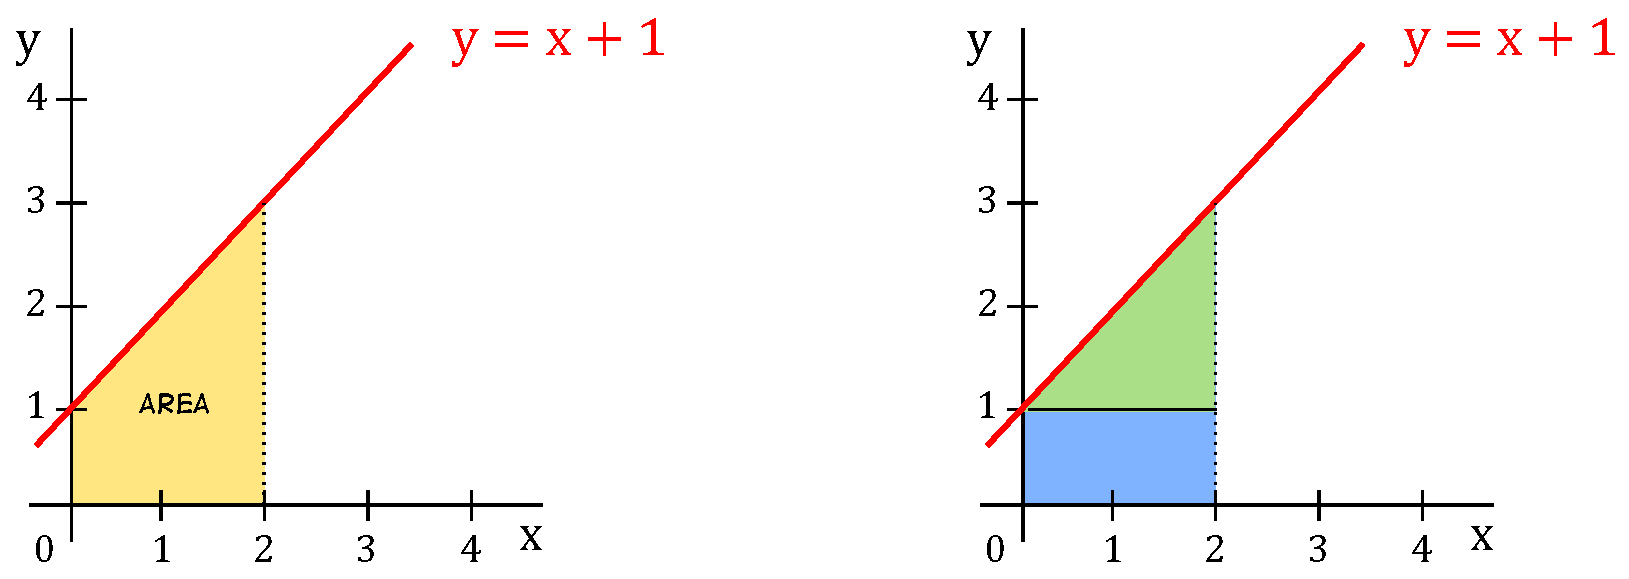
\includegraphics[width=5in]{images/int-ex}$$
Thus, the area is the sum of the areas of a rectangle and a triangle.
Hence,
\begin{eqnarray*}
\int_0^2 x+1~dx&=&\mbox{Net Area}\\
&=&\mbox{Area of rectangle} + \mbox{Area of triangle}\\
&=&(2)(1)+\frac{1}{2}(2)(2)\\
&=&4.
\end{eqnarray*}
\end{solution}

We next apply FTC to differentiate a function.

\begin{example}{Using FTC}{UsingFTC}
\exfont{Differentiate} the following function:
$$g(x)=\int_{-2}^x \cos(1+5t)\sin t\,dt.$$
\end{example}

\begin{solution} 
We simply apply the Fundamental Theorem of Calculus directly to get:
$$g'(x)=\cos(1+5x)\sin x.$$
\end{solution}

Using the Chain Rule we can derive a formula for some more complicated problems.
We have:
$$\frac{d}{dx}\int_a^{v(x)}f(t)\,dt=f(v(x))\cdot v'(x).$$

Now what if the upper limit is constant and the lower limit is a function of $x$?
Then we interchange the limits and add a minus sign to get:
$$\frac{d}{dx}\int_{u(x)}^af(t)\,dt=-\frac{d}{dx}\int_a^{u(x)} f(t)\,dt=-f(u(x))\cdot u'(x).$$

Combining these two we can get a formula where both limits are a function of $x$.
We break up the integral as follows:
$$\int_{u(x)}^{v(x)} f(t)\,dt=\int_{u(x)}^a f(t)\,dt+\int_a^{v(x)}f(t)\,dt.$$
We just need to make sure $f(a)$ exists after we break up the integral.
Then differentiating and using the above two formulas gives:

\begin{formulabox}[FTC I + Chain Rule:]
$$\frac{d}{dx}\int_{{u(x)}}^{{v(x)}} f(t)\,dt=f({v(x)}){v'(x)}-f({u(x)}){u'(x)}$$
\end{formulabox}

Many textbooks do not show this formula and instead to solve these types of problems will use FTC I along with the tricks we used to derive the formula above.
Either method is perfectly fine.

\begin{example}{FTC I + Chain Rule}{FTCIChainRule}
Differentiate the following integral:
$$\int_{10x}^{x^2} t^3\sin(1+t) \,dt.$$
\end{example}

\begin{solution} 
We will use the formula above.
We have $f(t)=t^3\sin(1+t)$, $u(x)=10x$ and $v(x)=x^2$.
Then $u'(x)=10$ and $v'(x)=2x$.
Thus,
\begin{eqnarray*}
\frac{d}{dx}\int_{10x}^{x^2} t^3\sin(1+t) \,dt&=&(x^2)^3\sin(1+(x^2))(2x)-(10x)^3\sin(1+(10x))(10)\\
\\
&=&2x^7\sin(1+x^2)-10000x^3\sin(1+10x)
\end{eqnarray*}
\end{solution}

\begin{example}{FTC I + Chain Rule}{FTCIChainRule2}
Differentiate the following integral with respect to $x$:
$$\int_{x^3}^{2x} 1+\cos t\,dt$$
\end{example}

\begin{solution} 
Using the formula we have:
$$\frac{d}{dx}\int_{x^3}^{2x} 1+\cos t\,dt=(1+\cos(2x))(2)-(1+\cos(x^3))(3x^2).$$
\end{solution}


%%%%%%%%%%%%%%%%%%%%%%%%%%%%%%%%%%%%%%%%%%%%%%%%%
\Opensolutionfile{solutions}[ex]
\section*{Exercises for Section \ref{sec:FTC}}

\begin{enumialphparenastyle}

%%%%%%%%%%
\begin{ex}
Evaluate $\ds \int_1^4 t^2+3t\,dt$
\begin{sol}
 $87/2$
\end{sol}
\end{ex}

%%%%%%%%%%
\begin{ex}
Evaluate $\ds \int_0^\pi \sin t\,dt$
\begin{sol}
 $2$
\end{sol}
\end{ex}

%%%%%%%%%%
\begin{ex}
Evaluate $\ds \int_1^{10} {1\over x}\,dx$
\begin{sol}
 $\ln(10)$
\end{sol}
\end{ex}

%%%%%%%%%%
\begin{ex}
Evaluate $\ds \int_0^5 e^x\,dx$
\begin{sol}
 $\ds e^5-1$
\end{sol}
\end{ex}

%%%%%%%%%%
\begin{ex}
Evaluate $\ds \int_0^3 x^3\,dx$
\begin{sol}
 $\ds 3^4/4$
\end{sol}
\end{ex}

%%%%%%%%%%
\begin{ex}
Evaluate $\ds \int_1^2 x^5\,dx$
\begin{sol}
 $\ds 2^6/6 -1/6$
\end{sol}
\end{ex}

%%%%%%%%%%
\begin{ex}
 Find the derivative of $\ds G(x)=\int_1^x t^2-3t\,dt$
\begin{sol}
 $\ds x^2-3x$
\end{sol}
\end{ex}

%%%%%%%%%%
\begin{ex}
 Find the derivative of $\ds G(x)=\int_1^{x^2} t^2-3t\,dt$
\begin{sol}
 $\ds 2x(x^4-3x^2)$
\end{sol}
\end{ex}

%%%%%%%%%%
\begin{ex}
 Find the derivative of $\ds G(x)=\int_1^x e^{t^2}\,dt$
\begin{sol}
 $\ds e^{x^2}$
\end{sol}
\end{ex}

%%%%%%%%%%
\begin{ex}
 Find the derivative of $\ds G(x)=\int_1^{x^2} e^{t^2}\,dt$
\begin{sol}
 $\ds 2xe^{x^4}$
\end{sol}
\end{ex}

%%%%%%%%%%
\begin{ex}
 Find the derivative of $\ds G(x)=\int_1^x \tan(t^2)\,dt$
\begin{sol}
 $\ds \tan(x^2)$
\end{sol}
\end{ex}

%%%%%%%%%%
\begin{ex}
 Find the derivative of $\ds G(x)=\int_{10x}^{x^2} \tan(t^2)\,dt$
\begin{sol}
 $\ds 2x\tan(x^4)-10\tan(100x^2)$
\end{sol}
\end{ex}

%%%%%%%%%%
\begin{ex}
Suppose $\int_{1}^{4}f(x)\,dx=2$ and $\int_{1}^{4}g(x)\,dx=7$. Find $\int_{1}^{4}(5f(x)+3g(x))\,dx$ and $\int_{1}^{4}(6-2f(x))\,dx$.
\begin{sol}
	31, 14
\end{sol}
\end{ex}

%%%%%%%%%%
\begin{ex}
Suppose $\int_{-2}^{5}f(x)\,dx=3$ and $\int_{1}^{5}f(x)\,dx=-2$. Find $\int_{-2}^{1}f(x)\,dx$.
\begin{sol}
	5
\end{sol}
\end{ex}

%%%%%%%%%%
\begin{ex}
If $f$ is continuous on $[a,b]$, we define the average of $f(x)$ on $[a,b]$ to be
\begin{equation*}
\text{avg}_{[a,b]}(f)=\frac{1}{b-a}\int_{a}^{b}f(x)\,dx.
\end{equation*}
\begin{enumerate}
	\item	What is the average of $\sqrt{x}$ on the interval $[0,1]?$
	\item	If the average of $f(x)$ on $[0,2]$ and on $[2,5]$ are 6 and 4 respectively, then what is its average on $[0,5]$?
\end{enumerate}
\begin{sol}
\begin{enumerate}
	\item	2/3
	\item	24/5
\end{enumerate}
\end{sol}
\end{ex}

\end{enumialphparenastyle}